\documentclass{statsmsc}

% Vim note: zo, zc and zm to open and close folds, and close all folds

% Commands {{{

\title{Title of the Thesis}
\author{FIRSTNAME LASTNAME}
\CID{01234567}
\supervisor{SUPERVISORNAME and COSUPERVISORNAME}
\date{1 May 2022}
%For today's date, use:
%\date{\today}
\logoimg{}


% THIS IS WHERE NEW COMMANDS CAN BE DEFINED
% commands below only used in the proof; otherwise can be deleted
\newcommand{\consta}{a}
\newcommand{\X}{X}
\newcommand{\EE}[1]{ \mathrm{E} [ #1 ] }
\newcommand{\inparenth}[1]{\left( #1 \right)}

% }}}

\begin{document}

%%%%% Heading %%%%%
% Heading {{{

% Generates the Title Page
\maketitle


% Generates plagiarism declaration
\declarationname{STUDENT'S NAME}
\declarationdate{DATE}
\declaration


\begin{abstract}
    ABSTRACT GOES HERE
\end{abstract}

\begin{acknowledgements}
    ANY ACKNOWLEDGEMENTS GO HERE
\end{acknowledgements}

{\thispagestyle{plain}
    \tableofcontents
}

% Glossary ?
{\chapter*{Notation}\thispagestyle{plain}
    $\boldsymbol{X}$ is a matrix

    $y$ is a vector
}

% Abbreviations
{\chapter*{Abbreviations}\thispagestyle{plain}
    \begin{acronym}[TDMA]
        \acro{DAIN}{Deep Adaptive Input Normalization}
        \acro{RDAIN}{Robust Deep Adaptive Input Normalization}
        \acro{EDAIN}{Extended Deep Adaptive Input Normalization}
        \acro{EDAIN-KL}{Extended Deep Adaptive Input Normalization, optimised with Kullback–Leibler divergence}
        \acro{BIN}{Bilinear Input Normalization}
        \acro{pdf}{probability density function}
        \acro{KL-divergence}{Kullbeck-Leibler divergence}
        \acro{PREPMIX-CAPS}{Preprocessing Mixture, optimised with Clustering and Parallel Seearch}
        \acro{API}{Application Programming Interface}
        \acro{GPU}{Graphics Processing Unit}
    \end{acronym}
}



% VERY IMPORTANT
% This command switches from Roman to Arabic numbering for main part of thesis
\mainmatter

% }}}

%%%%%%%%%%%%%%%%%%%%%%%%%%%%%%%%%%%%%%%%%%%%%%%%%%%%%%
\chapter{Introduction} %%%%     Introduction      %%%%
%%%%%%%%%%%%%%%%%%%%%%%%%%%%%%%%%%%%%%%%%%%%%%%%%%%%%%
% Introduction {{{

The introduction section goes here\footnote{Tip: write this section last.}.

% }}}

%%%%%%%%%%%%%%%%%%%%%%%%%%%%%%%%%%%%%%%%%%%%%%%%%%%%%%
\chapter{Background} %%%%        Background       %%%%
%%%%%%%%%%%%%%%%%%%%%%%%%%%%%%%%%%%%%%%%%%%%%%%%%%%%%%

TODO: introduction to this chapter

\section{Deep learning}% Deep learning
% Methods: Deep learning {{{
\label{sec:Deep learning}

TODO: write details

% TODO: stuff to mention
% * Backpropogation, weights
% * meaning of "forward" pass
% * "backwards" pass
% * What a GPU is, and how used to train models efficiently (nice to get this
%   mentioned, as PREPMIX optimisation part mentions distributing computation to
%   different GPUs)

\subsection{Sequence models}%
\label{sub:Sequence models}


% }}}

\section{Data preprocessing}% Data preprocessing
% Methods: Data preprocessing {{{
\label{sec:Data preprocessing}

Origin pa

\cite{stanislav} does some data preprocessing for neural networks, and
\cite{nawi} also investigate the effect of data preprocessing on neural network.
Also looked at effect on classification performance by \cite{singh}.
Moreover, been studied as early as 1997 by \citep{preprocess_origin}.

% Static distribution transformations
\subsection{Static distribution transformations}% {{{
\label{sub:Static distribution transformations}


% }}}

% Adaptive distribution transformation
\subsection{Adaptive distribution transformations}% {{{
\label{sub:Adaptive distribution transformations}

\subsubsection{DAIN}%
\label{ssub:DAIN}

The \ac{DAIN} method, proposed by \cite{dain}.

\subsubsection{RDAIN}%
\label{ssub:RDAIN}

We have \cite{rdain}

\subsubsection{BiN}%
\label{ssub:BiN}

We have \cite{bin}

% }}}


% }}}


\section{Normalizing flows}% Normalizing flows
% Methods: Normalizing flows {{{
\label{sec:Normalizing flows}

TODO: write details

% }}}


%%%%%%%%%%%%%%%%%%%%%%%%%%%%%%%%%%%%%%%%%%%%%%%%%
\chapter{Methods} %%%%       METHODS         %%%%
%%%%%%%%%%%%%%%%%%%%%%%%%%%%%%%%%%%%%%%%%%%%%%%%%

TODO: introduction to this chapter

\section{EDAIN}% EDAIN
% Methods: EDAIN {{{
\label{sec:EDAIN-method}

% Topics of this section:
% * Illustrative diagram of the 4 layers, and the weights, justifying order of operations
% * Differences to DAIN, explaining batch awareness, and specifics of (amex) dataset worked with
% * Explaining the 3 parts:
%   * outlier removal: Inspired by winsorization, plot of curve for different values,to show how work
%   * scale&shift: able to generalise standard scaling
%   * power transform: should also work for negative and positive values, while being numerically stable


% TODO: Replace this introduction with the architecture subsection
My first contribution is the \ac{EDAIN} layer. This adaptive preprocessing layer is inspired
by the likes of \citep{dain}  and \citep{bin} but unlike the aforementioned methods, the
\ac{EDAIN} layer also supports normalizing the data in a \textit{global-aware} fashion, whereas
the \ac{DAIN}, \ac{RDAIN} and \ac{BIN} layers are all \textit{local-aware}.
Additionally, the \ac{EDAIN} layer extends the other layers with two new operations: An outlier
removal operation that is designed to reduce the negative impact of high-tail observations,
as well as a power-transform operation that is designed to transform skewed data to be more
normal.

% TODO: move notation out of EDAIN section
\subsection{Notation}%
\label{sub:Notation}


Let $\{\bfX^{(i)} \in \R^{d \times T};i=1,\dots,N\}$ denote a set of $N$ multivariate time-series,
each composed of $T$ $d$-dimensional feature vectors. We also let $\bfx_t^{(i)}\in \R^d$,
where $t=1,\dots,T$, denote the $t$th feature vector at time-step $t$ in the time-series.
When talking about applying operations on feature vectors of the form $\bfx_t^{(i)}$, the time index and data index might
be dropped for notational clarity, giving $\bfx \in \R^d$. Furthermore, the vector operations
$\oplus, \ominus, \odot, \oslash$ refer to the element-wise
application of addition, subtraction, multiplication and division, respectively.

Something something vector function with vector input and vector output, is denoted with bold
letter such as $\mathbf{f}(\bfx)$, and functions applied elementwise is denoted $f(x)$.

\subsection{Architecture}%
\label{sub:Architecture}

% Latex equations used:
% \(\mathbf{\alpha}' \odot \left(\mathbf{\beta}' \odot \tanh\left\{(\mathbf{x}_t^{(i)}-\hat{\mathbf\mu}) \oslash \mathbf{\beta}'  \right\}+\hat{\mathbf\mu} \right)+\left(1-\mathbf{\alpha}' \right) \odot \mathbf{x}_t^{(i)}\)
% \((\mathbf{\tilde{x}}_t^{(i)}  - \mathbf{\gamma} \mathbf{\mu}_{\mathbf{\tilde{x}}_t^{(i)}}) \oslash \mathbf{\lambda} \sigma_{\mathbf{\tilde{x}}_t^{(i)}}, \textrm{ if local-aware} \)
% TODO: add w=(alpha, beta) above the red boxes to highlight which parameters are optimized...
\begin{figure}
\begin{center}
    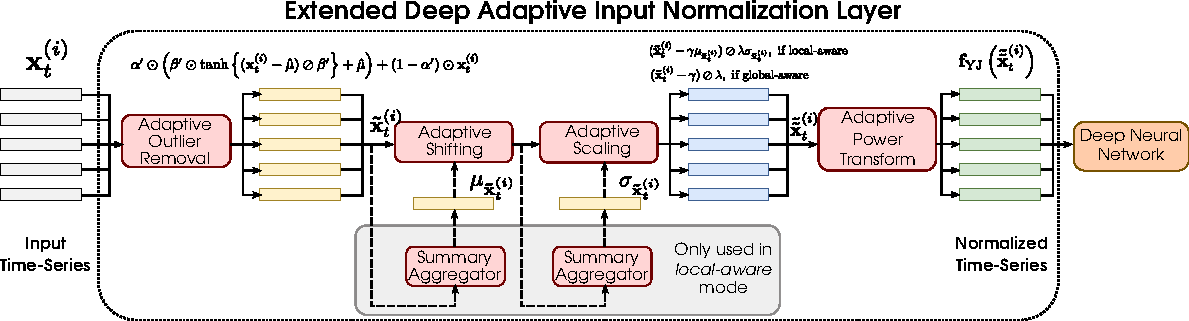
\includegraphics[width=\textwidth]{diagrams/edain-diagram.pdf}
\end{center}
\caption{An overview of the architecture of the proposed \ac{EDAIN} normalization layer.}
\label{fig:edain-arch}
\end{figure}

An overview of the layer's architecture is shown in figure \cref{fig:edain-arch}.
Given some input time-series $\bfX^{(i)} \in \R^{d \times T}$, each temporal segment
$\bfx^{(i)}_t$ is passed through an adaptive outlier removal layer, followed by an adaptive shift
and scale operation, and then finally passed through an adaptive power transformation layer.
The architecture also has two modes, \textit{local-aware} and \textit{global-aware}. In
global-aware mode, the \ac{EDAIN} layer aims to normalize each input such that the resulting
distribution of all the samples in the dataset resemble a unimodal normal distribution, that is
a ``global normalization''. In local-aware mode,
the \ac{EDAIN} layer's normalization operations
also depend on summary statistics of each input sample $\bfX^{(i)}$, and the goal is to transform
all the data into a common normalized representation space, independent of where in the
``global distribution'' the sample originated from. This mode is most suitable for
multi-modal input data, as samples from different modes can all be transformed into one common
normalized unimodal distribution. On the other hand, the global-aware mode
is most suitable if all the data comes from a similar data generation mechanism,
and works best if the input data has few modes.

In local-aware mode, the \ac{EDAIN} architecture is similar to the
\ac{DAIN} architecture proposed by \citeauthor{dain}, but it
extends it with both a global-aware mode as well as an adaptive outlier removal sublayer and
an adaptive power transform sublayer.

% Outlier removal
\subsubsection{Outlier removal}% {{{
\label{ssub:Outlier removal}

Handling outliers and extreme values in the dataset can increase predictive performance if done
correctly (citation needed). Two common ways of doing this are omission and winsorization
\citep{winsorization}. With the former, observations that are deemed to be extreme are simply
removed during training. With the latter, all the data is still used, but observations lying
outside a certain number of standard deviation from the mean, or below or above certain
percentiles, are \textit{clamped down} to be closer to the mean or median of the data.
For example, if winsorizing data using 3 standard deviation, all values less than
$\mu-3\sigma$ are set to be exactly $\mu-3\sigma$. Similarly, the values above
$\mu+3\sigma$ are \textit{clamped} to this value. Winsorization can also be done using percentiles,
where common boundaries are the first and fifth percentiles \citep{winsorization}.
However, the type of winsorization, as well as the number of standard deviation
or percentiles to use, might depend on the dataset. Additionally, it might not
be necessary to winsorize the data at all if the outliers turn out to not
negatively affect performance. All this introduces more hyperparameters to tune
during modelling. The outlier removal operation presented here aims to automatically  determine both
whether winsorization is necessary for a particular feature, and determine the threshold at
which to apply winsorization.

For input vector $\bfx_t^{(i)} \in \R^d$, the adaptive outlier removal operation is defined as:
\begin{equation}\label{eq:adaptive-outlier-removal}
    \mathbf{h}_1(\bfx_t^{(i)})=\bm\alpha' \odot \underbrace{\left(\bm\beta' \odot
        \tanh\left\{(\bfx_t^{(i)}-\hat{\bm\mu}) \oslash \bm\beta'  \right\}+\hat{\bm\mu}
\right)}_{\text{smooth adaptive centred winsorization}}
    +\underbrace{\left(1-\bm\alpha' \right) \odot \bfx}_{\text{residual connection}},
\end{equation}
where
$\bm\alpha' \in [0,1]^d$ is a parameter controlling how much winsorization to apply to each feature,
and $\bm\beta' \in [\beta_{\text{min}},\infty)^d$ controls the winsorization threshold for
each feature, that is, the maximum absolute value of the output, thus controlling the range of the
output. The effect of the two parameters is illustrated in \cref{fig:adaptive_outlier}.
The unknown parameters of the model are $\bm\alpha \in \R^d$ and $\bm\beta \in \R^d$, and they
are transformed into the constrained parameters $\bm\alpha'$ and $\bm\beta'$, as used in
\cref{eq:adaptive-outlier-removal} through the following element-wise mappings:
\begin{equation}
    \bm\alpha'=\frac{e^{\bm\alpha}}{1\oplus e^{\bm\alpha}} \qquad\qquad
    \bm\beta'=\beta_{\text{min}}\oplus e^{\bm\beta},
\end{equation}
where $\beta_{\textrm{min}} \in \R$ is a hyperparameter that can be tuned, but a suitable value is $\beta_{\textrm{min}}=1$.


The $\hat{\bm\mu}\in \R^d$ parameter in \cref{eq:adaptive-outlier-removal} is an estimate of the mean of the data, and is used
to ensure the winsorization is centred. When setting the \ac{EDAIN} layer in \textit{local-aware}
mode, it is simply the mean of the current batch of data points, $\mathcal{B}$:
\begin{equation}
    \hat{\mu}_k=\frac{1}{|\mathcal{B}| T} \sum_{i \in \mathcal{B}} \sum_{j=1}^T x_{j,k}^{(i)}, \qquad k=1,\dots,d
\end{equation}
while if using the \textit{global-aware} mode, it is iteratively updated using a cumulative
moving average estimate at each forward pass of the layer. This is to better approximate the
global mean of the data.
% For ease of notation, we let $\mathbf{W}_1=(\bm\alpha, \bm\beta)$ denote the $2d$ unknown
% parameters that are optimised for the adaptive outlier removal layer.

\begin{figure}
\begin{center}
    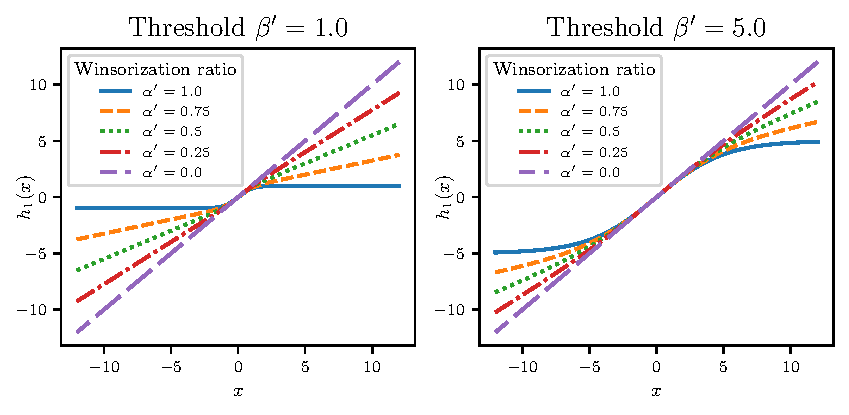
\includegraphics[scale=1.0]{figures/adaptive_outlier_removal.pdf}
\end{center}
\caption{Plot of the adaptive outlier removal operation for different combinations of parameter
values for $\alpha'$ and $\beta'$.}
\label{fig:adaptive_outlier}
\end{figure}


% }}}

% Scale and shift
\subsubsection{Scale and shift}% {{{
\label{ssub:Scale and shift}

Depending on the dataset, one might want to aim for a \textit{global
normalization}, in which case a \textit{global-aware} scale and shift operation is most
suitable. If the dataset has many different modes, with significantly different distribution characteristics, a \textit{local normalization} based on the specific mode each data point comes from is more suitable, in which case a \textit{local-ware} scale and shift
operation works best. This gives two different approaches and scaling and shifting the data in an adaptive fashion.

\paragraph{Global-aware}%
\label{par:Global-aware}

In global-aware mode, the adaptive shift and scale layer, combined, simply performs the operation
\begin{equation}\label{eq:adaptive-scale-shift}
    \mathbf{h}_3(\mathbf{h}_2(\bfx_t^{(i)})):=(\bfx_t^{(i)} - \bm\gamma) \oslash \bm\lambda,
\end{equation}
with input $\bfx \in \R^d$ and unknown parameters $\bm\gamma \in \R^d$ and $\bm\lambda \in (0,\infty)^d$.
This makes the scale-and-shift layer a generalised version of
Z-score scaling, or standard scaling, as setting
\begin{equation}
    \bm\gamma:=\frac{1}{N T}  \sum^{N}_{i=1} \sum^{T}_{t=1} \bfx_{t}^{(i)}
\end{equation}
and
\begin{equation}
    \bm\lambda:=\frac{1}{N T} \sum^{N}_{i=1} \sum^{T}_{t=1} \left(\bfx_{t}^{(i)}- \bm\gamma\right)^2
\end{equation}
makes the operation in \cref{eq:adaptive-scale-shift} equivalent to Z-score scaling.
This \textit{global-ware} mode is useful if the distribution is similar across batches
and constitute a global unimodal distribution that should be centred, as the operation can generalise Z-score scaling.

\paragraph{Local-aware}%
\label{par:Local-aware}

Some datasets might have multiple modes arising from significantly different
data generation mechanisms. Attempting to scale and shift each batch to a global mean and
standard deviation might hurt performance in such cases. Instead, \citeauthor{dain} propose
basing the scale and shift on a \textit{summary representation} of each data point, allowing
each sample to be normalized according the specific mode  of the data it might have come from.
This gives
\begin{equation}
    \mathbf{h}_3(\mathbf{h}_2(\bfx_t^{(i)})):=  (\bfx_t^{(i)} - [\bm\gamma \odot \mu_{\bfx}]) \oslash [\bm\lambda \odot \sigma_{\bfx}],
\end{equation}
where the summary representations $\sigma_{\bfx}$ and $\mu_{\bfx}$ are computed through reduction
of the temporal dimension for each observation:
\begin{align}
    \mu_\bfx^{(i)}&=\frac{1}{T} \sum^{T}_{t=1} \bfx^{(i)}_t \in \R^d \\
    \sigma_\bfx^{(i)}&=\sqrt{\frac{1}{T}  \sum^{T}_{t=1} \left(\bfx^{(i)}_t- \mu_\bfx^{(i)} \right)^2} \in \R^d.
\end{align}
With this mode, it is difficult for the layer to generalise Z-score scaling, but it allows
discarding mode information such that highly multimodal distributions appear unimodal.

% }}}

% Power transform
\subsubsection{Power transform}% {{{
\label{ssub:Power transform}

Many real-world datasets exhibit significant skewness, which is often treated using power
transformations (citation needed). The most common transformation is the Box-Cox transformation,
but this is only valid for positive values, so it is not applicable to most real-world datasets
\citep{boxcox}. An alternative is a transformation proposed by \citeauthor{yeoJohnson}
who proposed to following transformation:
\begin{equation}\label{eq:yeo-johnson}
    f_{\textrm{YJ}}(x)= \left\{
        \begin{array}{ll}
            \frac{(x+1)^{\lambda^{(\textrm{YJ})}}-1}{\lambda^{(\textrm{YJ})}}, & \textrm{if } \lambda^{(\textrm{YJ})} \neq 0, x \geq 0; \\
            \log(x + 1), & \textrm{if } \lambda^{(\textrm{YJ})} = 0, x \geq 0;  \\
            \frac{(1-x)^{2-\lambda^{(\textrm{YJ})}}-1}{\lambda^{(\textrm{YJ})}-2} , & \textrm{if } \lambda^{(\textrm{YJ})} \neq 2, x < 0; \\
            -\log(1-x), & \textrm{if } \lambda^{(\textrm{YJ})}=2, x < 0.
        \end{array}
    \right.
\end{equation}
Like the Box-Cox transformation, transformation $f_{\textrm{YJ}}$ only has one unknown parameter, $\lambda^{(\textrm{YJ})}$, but
it works for any $x \in \R$, not just positive values \citep{yeoJohnson}.
The power transform layer simply applies the transformation in \cref{eq:yeo-johnson} along each dimension of the input, that is for each $i=1,\dots,N$ and $t=1,\dots,T$,
\begin{equation}
    \left[\mathbf{h}_4\left(\bfx_t^{(i)}\right)\right]_j:=f_{\textrm{YJ}}(x_{t,j}^{(i)}), \;\;\; j=1,\dots,d.
\end{equation}
The unknown parameters is the vector $\bm\lambda^{(\textrm{YJ})} \in \R^d$.


% }}}

% Optimising the parameters
\subsection{Optimisation through back-propagation}% {{{
\label{sub:Optimising the parameters}

To optimise the unknown parameters
$\left( \bm{\alpha}, \bm{\beta}, \bm{\gamma}, \bm{\lambda}, \bm{\lambda}^{(\textrm{YJ})}\right)$,
the deep neural network is augmented by prepending the \ac{EDAIN} layer, as shown in
\cref{fig:edain-arch}. Then the input data is fed into the augmented model in batches,
as when training a neural network, and after each forward pass of the model, the weights
are updated through gradient descent while training the neural network.
As observed by \citeauthor{dain}, the model convergence is unstable if the same learning rate
$\eta \in \R$ that is used for training the deep neural network is also used for training all
the sublayers of the \ac{EDAIN} layer. Therefore, separate learning rate modifiers
$\eta_{\textrm{out}}$,
$\eta_{\textrm{shift}}$,
$\eta_{\textrm{scale}}$ and
$\eta_{\textrm{pow}}$ for the outlier removal, shift, scale and power transform sublayers are
introduced as additional hyperparameters and the weight updates happen according to the equation:
\begin{equation}
    \Delta \left( \bm{\alpha}, \bm{\beta}, \bm{\gamma}, \bm{\lambda}, \bm{\lambda}^{(\textrm{YJ})}\right)
    =
    -\eta\left(
        \eta_{\textrm{out}} \frac{\partial \mathcal{L}}{\partial \bm\alpha},
        \eta_{\textrm{out}} \frac{\partial \mathcal{L}}{\partial \bm\beta},
        \eta_{\textrm{shift}} \frac{\partial \mathcal{L}}{\partial \bm\gamma},
        \eta_{\textrm{scale}} \frac{\partial \mathcal{L}}{\partial \bm\lambda},
        \eta_{\textrm{pow}} \frac{\partial \mathcal{L}}{\partial \bm{\lambda}^{(\textrm{YJ})}}
    \right).
\end{equation}


% }}}

% }}}

\section{EDAIN-KL}% EDAIN-KL
% Methods: EDAIN-KL {{{
\label{sec:EDAIN-KL-method}

TODO: introduction
something something alterative inspired by normalizing flow, and mention bijectors.

\subsection{Architecture}%
\label{sub:Architecture}

The \ac{EDAIN-KL} layer has a very similar architecture to the \ac{EDAIN} layer, described in
\cref{sec:EDAIN-method}, but the outlier removal transformation has been simplified to ensure its
inverse is tractable. Additionally, the layer no longer supports local-aware mode, as this
would make the inverse intractable. The \ac{EDAIN-KL} transformations are:
\begin{align}
    \textrm{(Outlier removal)} \qquad& \mathbf{h}_1\left(\bfx^{(i)}_t\right)=\bm\beta' \odot \tanh\left\{(\bfx^{(i)}_t - \hat{\bm\mu}) \oslash \bm\beta' \right\}+\hat{\bm\mu} \label{eq:kl1}\\
    \textrm{(shift)} \qquad& \mathbf{h}_2\left(\bfx^{(i)}_t\right)=\bfx^{(i)}_t\oplus \bm\gamma \label{eq:kl2}\\
    \textrm{(scale)} \qquad& \mathbf{h}_3\left(\bfx^{(i)}_t\right)=\bfx^{(i)}_t \odot \bm\lambda  \label{eq:kl3}\\
    \textrm{(power transform)} \qquad& \mathbf{h}_4\left(\bfx^{(i)}_t\right)=\left[
        f^{\lambda_1}_{\textrm{YJ}}\left(x^{(i)}_{t,0}\right)
        \quad f^{\lambda_2}_{\textrm{YJ}}\left(x^{(i)}_{t,1}\right)
        \quad \cdots
        \quad f^{\lambda_d}_{\textrm{YJ}}\left(x^{(i)}_{t,d}\right)
    \right], \label{eq:kl4}
\end{align}
where $f^{\lambda_i}_{\textrm{YJ}}(\cdot)$ is defined in \cref{eq:yeo-johnson}.

% TODO: explain how these functions are composed in the forward transformed, and how the thing is
%       inverted, and also overview of the inverse thing and how normalizing flow works
%       Idea, overview of how it's optimised and how data transformed back into normal using
%       change of variable formula. Goal is leading into why we need the derivations for ILDJs
\subsection{Optimisation through Kullback-Leibler divergence}%
\label{sub:Optimisation through Kullback-Leibler divergence}

This optimisation method is inspired by normalizing flow, of which \citeauthor{normalizing_flows}
provide a great overview of.

\subsubsection{Brief background on normalizing flow}%
\label{ssub:Brief background on normalizing flow}

Consider a random variable $\bfZ \in \R^d$ with a known and
analytic expression for the \ac{pdf} $p_\bfz: \R^d \rightarrow {\R}$, which we
call the \textit{base distribution}. The idea behind normalizing flows is
defining a arbitrarily complicated parametrised bijector
$\mathbf{g}_{\bm \theta}:\R^d \rightarrow {\R^d}$---an
invertible function---and transforming the simple base distribution into a new
arbitrarily complicated probability distribution: $\bfY=\mathbf{g}_{\bm\theta}(\bfZ)$.
The \ac{pdf} of the transformed distribution can then be computed using the change of variable
formula \citep{normalizing_flows}:
\begin{align}
    p_\bfY(\bfy)&=p_\bfZ(\mathbf{g}_{\bm\theta}^{-1}\left(\bfy\right))\cdot \left|\det \mathbf{J}_{\bfY \rightarrow {\bfZ}}\left(\bfy \right) \right| \nonumber \\
                & = p_\bfZ(\mathbf{g}_{\bm\theta}^{-1}\left(\bfy\right))\cdot \left|\det \mathbf{J}_{\bfZ \rightarrow {\bfY}}\left( \mathbf{g}^{-1}_{\bm\theta}(\bfy) \right) \right|^{-1},
\end{align}
where $\mathbf{J}_{\bfZ \rightarrow {\bfY}}$ is the Jacobian matrix for the forward mapping $\bfY = \mathbf{g}_{\bm\theta}(\bfZ)$.
Taking logs on both sides, it follows that
\begin{equation}\label{eq:logDetJac}
    \log p_\bfY(\bfy)= \log p_\bfZ(\mathbf{g}_{\bm\theta}^{-1}\left(\bfy\right)) - \log \left|\det \mathbf{J}_{\bfZ \rightarrow {\bfY}}\left(\mathbf{g}_{\bm\theta}^{-1}\left(\bfy\right) \right) \right|.
\end{equation}

One common application of normalizing flows is density estimation \citep{normalizing_flows};
Given a dataset $\mathcal{D}=\{\bfy^{(i)}\}_{i=1}^N$ with samples from some
unknown complicated distribution, we want to estimate its unknown \ac{pdf}, $p_{\mathcal{D}}$.
This can be done with likelihood-based estimation, where we assume the data points come from
parametrised distribution $\bfY=\mathbf{g}_{\bm \theta}(\bfZ)$ and optimise $\bm\theta$ to maximise
the data log-likelihood:
\begin{align}
    \log p(\mathcal{D}| \bm\theta)
    & = \sum_{i=1}^N \log p_\bfY(\bfy^{(i)}| \bm\theta ) \\
    &\stackrel{\cref{eq:logDetJac}}{=} \sum^{N}_{i=1}
    \log p_\bfZ\left(\mathbf{g}_{\bm\theta}^{-1}\left(\bfy^{(i)}\right)\right) - \log \left|\det \mathbf{J}_{\bfZ \rightarrow {\bfY}}\left(\mathbf{g}_{\bm\theta}^{-1}\left(\bfy^{(i)}\right)\right) \right|. \label{eq:logProbKL}
\end{align}
This is equivalent to minimising the \ac{KL-divergence} between the empirical distribution
$\mathcal{D}$ and the transformed distribution $\bfY=\mathbf{g}_{\bm\theta}(\bfZ)$:
\begin{align}
    \argmax_{\bm\theta} \log p(\mathcal{D}| \bm\theta)
    &= \argmax_{\bm\theta}\sum_{i=1}^N \log p_\bfY \left(\bfy^{(i)}\big|\bm\theta \right) \\
    &=\frac{1}{N}  \sum_{i=1}^N \log p_{\mathcal{D}}\left(\bfy^{(i)}\right)
        +\argmax_{\bm\theta}\frac{1}{N} \sum_{i=1}^N \log p_\bfY \left(\bfy^{(i)}\big|\bm\theta \right) \\
    &= \argmin_{\bm\theta}\frac{1}{N}  \sum_{i=1}^N \log p_{\mathcal{D}}\left(\bfy^{(i)}\right)
    -\frac{1}{N} \sum_{i=1}^N \log p_\bfY \left(\bfy^{(i)}\big|\bm\theta \right) \\
    &= \argmin_{\bm\theta}\sum^{N}_{i=1}  p_\mathcal{D}\left(\bfy^{(i)}\right)  \log p_{\mathcal{D}}\left(\bfy^{(i)}\right) \\
    &\qquad- \sum_{i=1}^N  p_\mathcal{D}\left(\bfy^{(i)}\right) \log p_\bfY \left(\bfy^{(i)}\big|\bm\theta \right) \\
    &= \argmin_{\bm\theta} D_{\textrm{KL}}\left(\mathcal{D}\;||\; (\bfY\mid\bm\theta)\right).
\end{align}
When training an normalizing flow model, we adjust $\bm\theta$ to minimize the
above \ac{KL-divergence}. This requires computing all the terms in \cref{eq:logProbKL}, which
requires analytic and differentiable expressions for the inverse transformation
$\mathbf{g}_{\bm\theta}^{-1}\left(\cdot \right)$, the \ac{pdf} of the base distribution
$p_{\bfZ}(\cdot)$ and the log determinant of the Jacobian matrix for $\mathbf{g}_{\bm\theta}^{-1}$,
$\log \left|\det \mathbf{J}_{\bfZ \rightarrow {\bfY}} \right|$. Using a result
stated in \citeauthor{normalizing_flows}, the following can be shown:
\begin{theorem}\label{thrm:normFlow}
    Let $\mathbf{g}_1,\dots, \mathbf{g}_n:\R^d \rightarrow {\R^d}$ all be bijective functions, and consider
    the composition of these functions, $\mathbf{g}=\mathbf{g}_n \circ \mathbf{g}_{n-1} \cdots \circ \mathbf{g}_1$.
    Then, $\mathbf{g}$ is a bijective function with inverse
    \begin{equation}
        \mathbf{g}^{-1}=\mathbf{g}_1^{-1} \circ \cdots \circ \mathbf{g}_{n-1}^{-1} \circ \mathbf{g}_n^{-1},
    \end{equation}
    and the log of the absolute value of the determinant of the Jacobian is given by
    \begin{equation}
        \log \left| \det \mathbf{J}_{\mathbf{g}^{-1}}(\cdot)\right|
        = \sum_{i=1}^N \log\left|\det \mathbf{J}_{\mathbf{g}_i^{-1}}(\cdot) \right|.
    \end{equation}
    Similarly,
    \begin{equation}
        \log \left| \det \mathbf{J}_{\mathbf{g}}(\cdot)\right|
        = \sum_{i=1}^N \log \left|\det \mathbf{J}_{\mathbf{g}_i}(\cdot) \right|.
    \end{equation}
\end{theorem}

\subsubsection{Application to EDAIN-KL}%
\label{ssub:Application to EDAIN-KL}

% TODO: here, provide some overview, including
% * choice of base distribution and how tractable
% * why we need to log det jacobians, but derivations in next section
% * how we get the inverses, and they are just the h_1 as shown in those equations...
Like with the \ac{EDAIN} layer, we want to compose the outlier removal, shift, scale and power
transform transformations into one operation, which we do by defining
\begin{equation}\label{eq:gtheta}
    \mathbf{g}_{\bm\theta}=\mathbf{h}_1^{-1} \circ  \mathbf{h}_2^{-1} \circ \mathbf{h}_3^{-1} \circ \mathbf{h}_4^{-1},
\end{equation}
where $\bm\theta=(\bm\beta, \bm\gamma, \bm\lambda, \bm\lambda^{(\textrm{YJ})})$.
Notice that we apply all the operations in reverse order, compared to the \ac{EDAIN} layer. This
is because we will use $\mathbf{g}_{\bm\theta}$ to transform our base distribution $\bfZ$ into
a distribution that is as close to our dataset $\mathcal{D}$ as possible. Then, when we want to
normalize the dataset, we apply
\begin{equation}\label{eq:gthetainv}
    \mathbf{g}_{\bm\theta}^{-1}=h_4 \circ h_3 \circ h_2 \circ h_1
\end{equation}
to each sample.  It can be shown that all the transformations defined in
\cref{eq:kl1,eq:kl2,eq:kl3,eq:kl4} are invertible. Using \cref{thrm:normFlow}, it follows that
$\mathbf{g}_{\bm\theta}$, as defined in \cref{eq:gtheta}, is bijective and that its inverse
is given by \cref{eq:gthetainv}. As we will see in later in \cref{ssub:ildj},
the inverse transformation in \cref{eq:gthetainv} has a tractable and differentiable expression,
so $\mathbf{g}_{\bm\theta}$ can be used as a normalizing flow bijection.

Making the input data as Gaussian as possible usually increases performance of deep sequence models
(citation needed), so a suitable base distribution is the standard multivariate Gaussian distribution
\begin{equation}
    \bfZ \sim \mathcal{N}(0, \mathbf{I}_d),
\end{equation}
whose \ac{pdf} has a tractable and differentiable expression, so it is suitable for our needs.

% TODO: change mentions of tractable to "analytic" as it makes more sense...
We have that both $p_\bfZ(\cdot)$ and $\mathbf{g}_{\bm\theta}^{-1}(\cdot)$ have analytic expressions
and are differentiable, so we have almost everything that we need in order to use
\cref{eq:logProbKL} to optimise $\bm\theta$. The only part remaining is an expression for
the log of the determinant of the Jacobian of the forward transformation given by
$\mathbf{g}_{\bm\theta}^{-1}$, which we will derive in the next section. Once we have that,
$\bm\theta$ can be optimised using back-propagation as described in TODO, using the negation
of \cref{eq:logProbKL} as the loss function $\mathcal{L}(\bm\theta)$.

\subsubsection{Derivations of inverse log determinant Jacobians}%
\label{ssub:ildj}

Recall that the \ac{EDAIN-KL} architecture is just a bijector that is composed of 4 other bijective
functions. Using the result in \cref{thrm:normFlow}, we get
\begin{equation}
    \log \left|\det \mathbf{J}_{\bfZ \rightarrow {\bfY}}(\cdot)  \right|
    = \sum^{4}_{i=1} \log \left|\det \mathbf{J}_{h_i^{-1}}(\cdot) \right|.
\end{equation}
Considering the transformations in \cref{eq:kl1,eq:kl2,eq:kl3,eq:kl4}, we notice that all the
transformation happen element-wise, so for $i\in\{1,2,3,4\}$, we have
$\frac{\partial h_i^{-1}(x_{j})}{\partial x_{k}} =0$ for $k \neq j$.
Therefore, the Jacobians are diagonal matrices, so the determinant is just the product of the
diagonal entries, giving
% TODO: below does not makes sense notaion-wise because h_i is not defined, since it's a vector function
\begin{align}
    \log \left|\det \mathbf{J}_{\bfZ \rightarrow {\bfY}}(\bfx)  \right|
    & = \sum^{4}_{i=1} \log \left| \prod_{j=1}^d \frac{\partial h_i^{-1}(x_j)}{\partial x_j}   \right| \\
    & = \sum^{4}_{i=1} \sum_{j=1}^d \log \left| \frac{\partial h_i^{-1}(x_j)}{\partial x_j}   \right|.
\end{align}

We now proceed to deriving the derivatives appearing on the right-hand side for
$h_1^{-1}$, $h_2^{-1}$, $h_3^{-1}$, and $h_4^{-1}$.

\paragraph{Shift}%
\label{par:Shift}

We first consider $h_2(x_j;\gamma_j)=x_j+\gamma_j$. Its inverse is $h_2^{-1}(z_j;\gamma_j)=z_j-\gamma_j$, and it follows that
\begin{equation}
    \log \left|\frac{\partial h_2^{-1}(z_j ; \gamma_j)}{\partial z_j} \right|
    = \log 1 = 0.
\end{equation}

\paragraph{Scale}%
\label{par:Scale}

We now consider $h_3(x_j;\lambda_j)=x_j\cdot \lambda_j$, whose inverse is $h_3^{-1}(x_j;\lambda_j)=\frac{z_j}{\lambda_j}$. It follows that
\begin{equation}
    \log \left|\frac{\partial h_3^{-1}(z_j ; \gamma_j)}{\partial z_j} \right|
    = \log \left|\frac{1}{\lambda_j}  \right|
    =- \log |\lambda_j|.
\end{equation}

\paragraph{Outlier removal}%
\label{par:Outlier removal}

We now consider $h_1(x_j;\beta'_j)= \beta'_j \tanh\left\{\frac{(x_j - \hat{\mu}_j)}{\beta'_j}  \right\} + \hat{\mu}_j$. Its inverse is
\begin{equation}
    h_1^{-1}(z_j;\beta_j') =\beta' \tanh^{-1} \left\{\frac{z_j - \hat{\mu}_j}{\beta'_j}  \right\}
    +\hat{\mu}_j.
\end{equation}
It follows that
\begin{equation}
    \log \left|\frac{\partial h_1^{-1}(z_j ; \beta_j')}{\partial z_j} \right|
    = \log \left| \frac{1}{1-\left( \frac{z_j-\hat{\mu}_j}{\beta_j'}  \right)^2}  \right|
    = -\log\left| 1-\left( \frac{z_j-\hat{\mu}_j}{\beta_j'}  \right)^2 \right|.
\end{equation}

\paragraph{Power transform}%
\label{par:Power transform}

By considering the expression in \cref{eq:kl4}, it can be shown that for fixed $\lambda$, negative inputs are always
mapped to negative values and vice versa, making the Yeo-Johnson transformation invertible.
Additionally, in $\mathbf{h}_4(\cdot)$ the Yeo-Johnson transformation is applied element-wise, so
we get
\begin{equation}
    \mathbf{h}_4^{-1}(\mathbf{z})=\left[\left[f_{\textrm{YJ}}^{\lambda_1}\right]^{-1}(z_1) \quad \left[f_{\textrm{YJ}}^{\lambda_2}\right]^{-1}(z_2) \quad \cdots \quad \left[f_{\textrm{YJ}}^{\lambda_d}\right]^{-1}(z_d) \right],
\end{equation}
where it can be shown that the inverse Yeo-Johnson transformation for a single element is given by
\begin{equation}
    \left[f_{\textrm{YJ}}^\lambda\right]^{-1}(z)= \left\{
    \begin{array}{ll}
        (z \lambda + 1)^{1/\lambda} -1, & \textrm{if } \lambda \neq 0, z \geq 0; \\
        e^z-1, & \textrm{if } \lambda = 0, z \geq 0;  \\
        1-\left\{1-z(2-\lambda)\right\}^{1/ (2-\lambda)} , & \textrm{if } \lambda \neq 2, z < 0; \\
        1-e^{-z}, & \textrm{if } \lambda=2, z < 0.
    \end{array}
    \right.
\end{equation}

The derivative with respect to $z$ then becomes
\begin{equation}
    \frac{\partial \left[f_{\textrm{YJ}}^\lambda\right]^{-1}(z)}{\partial z}= \left\{
        \begin{array}{ll}
            (z \lambda + 1)^{(1-\lambda)/\lambda}, & \textrm{if } \lambda \neq 0, z \geq 0; \\
            e^z, & \textrm{if } \lambda = 0, z \geq 0;  \\
            \left\{1-z(2-\lambda)\right\}^{(\lambda-1)/(2-\lambda)} , & \textrm{if } \lambda \neq 2, z < 0; \\
            e^{-z}, & \textrm{if } \lambda=2, z < 0.
        \end{array}
    \right.
\end{equation}
It follows that
\begin{equation}
    \log \left|\frac{\partial \left[f_{\textrm{YJ}}^\lambda\right]^{-1}(z)}{\partial z} \right|= \left\{
        \begin{array}{ll}
            \frac{1-\lambda}{\lambda}\log (z \lambda + 1), & \textrm{if } \lambda \neq 0, z \geq 0; \\
            z, & \textrm{if } \lambda = 0, z \geq 0;  \\
            \frac{\lambda - 1}{2-\lambda}\log\left\{1-z(2-\lambda)\right\} , & \textrm{if } \lambda \neq 2, z < 0; \\
            -z, & \textrm{if } \lambda=2, z < 0,
        \end{array}
    \right.
\end{equation}
which we use as the expression for $\log \left| \frac{\partial h_4^{-1}(z_j;\lambda^{(\textrm{YJ})})}{\partial z_j} \right|$ for $z=z_1,\dots,z_d$.

% }}}

\section{PREPMIX-CAPS}% PREPMIX-CAPS
% Methods: PREPMIX-CAPS {{{
\label{sec:PREPMIX-CAPS}

TODO: introduction to this method, and overview of how all the below subsections tie together
in the final method


\subsection{Clustering the predictor variables}%
\label{sub:prepmix-clustering}

% TODO: rephrase motivation of this paragraph
The input to this procedure is a tensor $\bfX \in \R^{N \times T \times d}$, containing $N$
multivariate time-series, each of length $T$ and containing $d$ numeric features.
In the clustering step, we want to cluster the features $\{1,2,3,\dots,d\}$ into $k$ disjoint groups,
such that the distribution of variables in each cluster has as similar characteristics as possible.
That way, applying the same preprocessing method to these variables might increase performance.
To achieve a clustering where the distribution characteristics within each clusters is as similar
as possible, I propose two approaches: One based on distribution statistics, and one information
theoretic approach.

\subsubsection{Clustering based on statistics}%
\label{sub:Clustering based on statistics}

% TODO: clean up writing, as this is not very nice to read...
The first clustering approach is based on statistics. With this approach, we first compute
$d_{\textrm{stats}}$ different statistics for each of the $d$ predictor variables in the tensor
$\bfX$. This then gives a $\bfX' \in \R^{d \times d_{\textrm{stats} }}$ matrix that can be used
to cluster the predictor variables later. The first statistic used is the Fisher's moment
coefficient of skewness \citep{shape}, which for $k=1,2,\dots,d$ is computed as
\begin{equation}\label{eq:fglkhy809s}
    \gamma_k=\frac{m_3}{m_2^{3/2}}, \quad \textrm{where }
    m_i=  \frac{1}{NT} \sum^{N}_{i=1} \sum^{T}_{t=1} \left(x^{(i)}_{t,k}-\mu_k \right)^i,
\end{equation}
where $\bm{\mu}=\frac{1}{NT}\sum^{N}_{i=1} \sum^{T}_{t=1} \bfx^{(i)}_t$ is the mean for each dimension. The second statistic used is the kurtosis \citep{shape}, which for $k=1,2,\dots,d$ is computed as
\begin{equation}
    \alpha_k=\frac{m_4}{m_2^2},
\end{equation}
where $m_i$ for $i\in \{2,4\}$ is defined in  \cref{eq:fglkhy809s}.
The third statistic used is the standard deviation, computed as
\begin{equation}
    \sigma_k=\sqrt{m_2},
\end{equation}
where $m_2$ is defined in \cref{eq:fglkhy809s}.

The next three statistics are based on binning, $\mathbf{B} \in \R^{d \times \textrm{num. bins}}$,
where $B_{k,i}$ denotes the number of samples from the set corresponding to the
$k$th predictor, $\left\{x_{t,k}^{(i)} \right\}_{i=1,\dots,N,\;t=1,\dots,T}$
that fall into the $i$th bin, all after applying min-max scaling of $[0,1]$ on the feature
space. The fourth statistic is computed as
\begin{equation}
    \frac{1}{n_{\textrm{num. bins} }}  \argmax_{i} B_{k,i},
\end{equation}
which models the location of the highest mode.
The fifth static is computed as
\begin{equation}
    \frac{1}{n_{\textrm{num. bins} }}  \sum^{n_{\textrm{num. bins} }}_{i=1} \mathbb{I}\left\{
        B_{k,i} > 0
    \right\},
\end{equation}
approximating how many unique values the distribution has. The sixth statistic is computed as
\begin{equation}
     \max_{i} B_{k,i},
\end{equation}
denoting the density in the highest mode.
After computing all the statistics and compiling the $\bfX' \in \R^{d \times d_{\textrm{stats} }}$,
here with $d_{\textrm{stats}}=6$, we apply $K$-means clustering on the matrix to get $k$ clusters
of the $d$ predictor \citep{kmeans}.

\subsubsection{Clustering based on KL-divergence}%
\label{sub:Clustering based on KL-divergence}

The second clustering method is based on information theory. We want to minimize the KL-divergence
between variables within the same cluster, which we can do by constructing a
distance matrix $\mathbf{W} \in \R^{d \times d}$ where $W_{i,j}$ denotes the
\ac{KL-divergence} between variable $j$ and $i$ for $j > i$, that is
from \citep{mackay} we set
\begin{equation}
    W_{i,j}= \sum^{n_{\textrm{num. bins} }}_{k=1} \mathbb{P}_{X_i}\left( \frac{k}{n_{\textrm{num. bins} }}  \right)
    \log\left\{
    \mathbb{P}_{X_i}\left( \frac{k}{n_{\textrm{num. bins} }}  \right) \bigg/
    \mathbb{P}_{X_j}\left( \frac{k}{n_{\textrm{num. bins} }}  \right)
\right\},
\end{equation}
where $\mathbb{P}_{X_i}(\cdot)$ is an approximation of the \ac{pdf} of the $i$th predictor variable,
which is approximated on support $[0,1]$ using a histogram of the $N \cdot T$ samples.

This distance matrix $\mathbf{W}$ is then used together with an agglomerative clustering approach
to cluster the $d$ variables into $k$ clusters
\citep{hierarchical_clustering}. Since the distance matrix $\mathbf{W}$ is
non-Euclidean, the linkage criteria used was selected to be ``average''.


\subsection{Determining the optimal preprocessing method for each cluster}%
\label{sub:Determining the optimal preprocessing method for each clusterch cluster}

\begin{figure}
    \begin{center}
        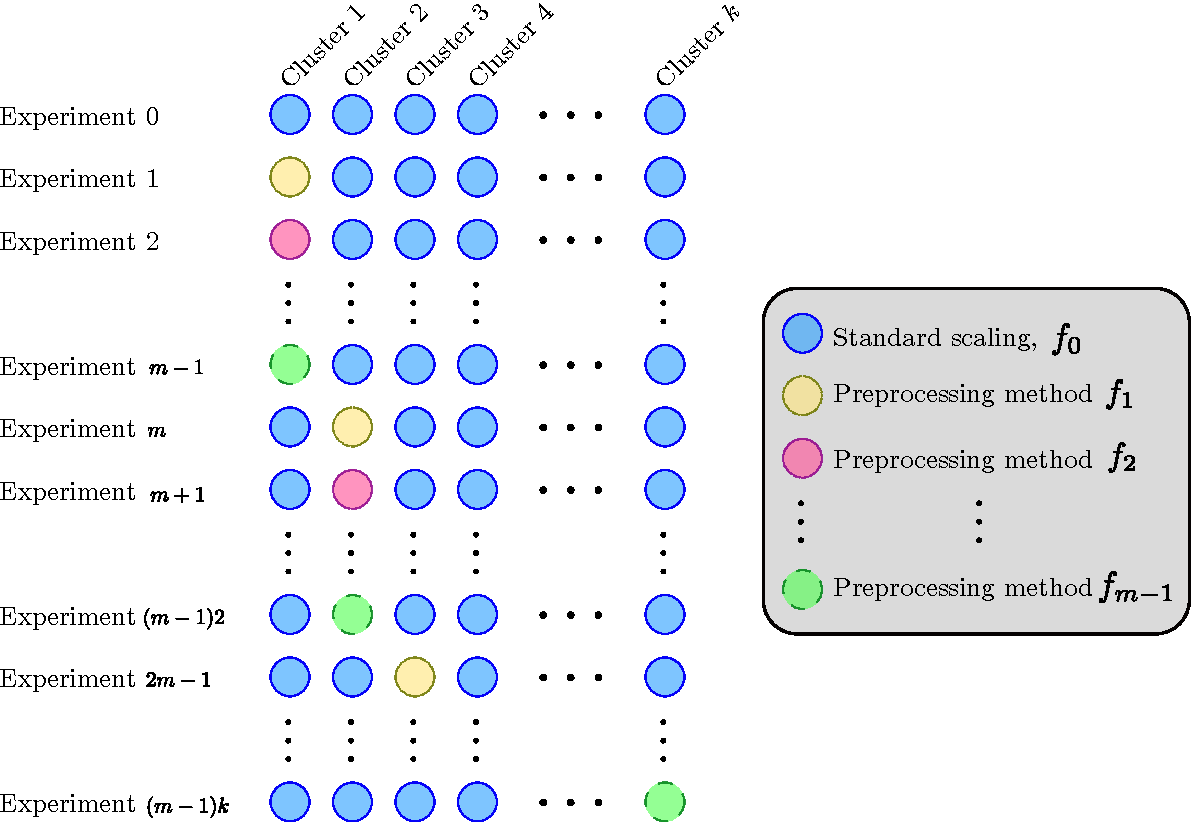
\includegraphics[width=\textwidth]{diagrams/prepmix-diagram.pdf}
    \end{center}
    \caption{Illustration of ``ablation studies'' done for finding the optimal preprocessing method
    for each cluster, as part of the \ac{PREPMIX-CAPS} routine.}
    \label{fig:prepmix}
\end{figure}

The goal of the \ac{PREPMIX-CAPS} preprocessing approach is preprocessing the
data using the mixture of preprocessing technique that gives the best
performance according to some validation metric. Usually, this is the
validation loss of the neural network being trained. As such, to select which
of the $f_0, f_1,\dots,f_{m-1}$ preprocessing techniques to apply to each
cluster, we try different combinations of preprocessing techniques and select
the transformation that gives the lowest validation loss for each cluster,
which requires training the model on the training data for each combination of
preprocessing techniques.  After clustering, we have $m$ different
preprocessing methods we consider for each cluster. Trying all of the possible
combinations would require training the neural network $m^k$ times, which is
computationally infeasible for large $k$ or $m$, especially of model training
is slow. Instead, we iteratively look at the isolated effect each of the
different preprocessing techniques have on a particular cluster, and repeat
this $k$ times, similar to an ablation study. For the clusters not being
considered in a particular experiment, a baseline preprocessing technique such
as standard scaling is applied to that cluster, as this technique in general
works well for most datasets (citation needed). This scheme reduces the number
of experiments from $m^k$ to $(m-1)k+1$, as we also do one experiment where the
baseline preprocessing technique is applied to all clusters. The scheme is
illustrated in \cref{fig:prepmix}, where we picked standard scaling as the
baseline preprocessing technique.

After these $(m-1)k+1$ experiments have been run, and the final validation loss has be recorded
for each experiment, say let $\mathcal{L}_{C_{i},f_j}$ denote the validation loss when running
the experiment for cluster $C_i$ where preprocessing method $f_j$ is used with $j>0$.
See \cref{fig:prepmix} for reference. For $C_1,\dots,C_k$, the validation loss
$\mathcal{L}_{C_i,f_0}$ is the validation loss from experiment 0, the baseline experiment.
Then, the preprocessing method for cluster $C_i$ is set to be $f_{\widehat{j}}$, where
\begin{equation}
    \widehat{j}=\argmin_{0 \leq j < m}  \mathcal{L}_{C_i,f_j}.
\end{equation}
This way of selecting the overall mixture based on local optimally techniques makes the assumption
that an isolated improvement in performance for a subset of the features generalise to overall
improvement in performance when combined with other features that might be preprocessing in a
different way.

\subsubsection{Optimisations}%
\label{ssub:Optimisations}

The different experiments, as shown in \cref{fig:prepmix}, have no dependencies
between them and can thus be executed in parallel. This allows optimising the
experiment running phase through parallel computation, as the computer the experiments were to
be run on had several cores as well as multiple \acp{GPU}. Before starting, the set of \acp{GPU}
to use has to be configured, denoted $\mathcal{I}_{\textrm{device IDs}}$ and the number of jobs
to run concurrently on each \ac{GPU} at any point in time, denotes $n_{\textrm{num. jobs}}$.
Then, all the experiments, or jobs, were abstracted away in a Python
\texttt{threading.Thread} object. The jobs were then allocated to the \acp{GPU} in
$\mathcal{I}_{\textrm{device IDs}}$ in a \textit{round-robin} fashion, that is, allocate the first
job to the first \ac{GPU}, the second job to the second \ac{GPU}, etc., going back to the first
\ac{GPU} once we reach the last \ac{GPU}. This is done until up to
$\# \mathcal{I}_{\textrm{device IDs}} \cdot n_{\textrm{num. jobs}}$ have been allocated and
set to execute. When these jobs finish, the subsequent experiments to run are scheduled in a similar
fashion. Unlike standard \textit{round-robin} scheduling, each job is run until completion instead
of switching while they execute.

\subsection{Hyperparameters}%
\label{sub:Hyperparameters}

For my experiments, I used the following selection of preprocessing techniques:
\begin{itemize}
    \item Standard scaling across both temporal axis and sample axis
    \item Standard scaling just across sample axis
    \item Standard scaling followed by $\tanh(\cdot)$ across both temporal axis and sample axis
    \item Standard scaling followed by $\tanh(\cdot)$ across sample axis
    \item Min-Max scaling to $[0,1]$ across both temporal axis and sample axis
    \item Min-Max scaling to $[0,1]$ across sample axis
\end{itemize}
This gives $m=5$. From hyperparameter tuning on $k$, also found $k=20$ for amex dataset
(TODO: don't go into datasets yet...).
For both clustering methods, the number of bins parameter, required for computing some of the
statistics, as well as estimating the \ac{pdf} values required for estimating the
\ac{KL-divergence} between the random variables, was set to be
$n_{\textrm{num. bins}}=5000$. The number of clusters $k$ to use, was tuned using the specific
dataset the \ac{PREPMIX-CAPS} method was applied to, which is described in section TODO.

% }}}

%%%%%%%%%%%%%%%%%%%%%%%%%%%%%%%%%%%%%%%%%%%%%%%%%%
\chapter{Results} %%%%         Results        %%%%
%%%%%%%%%%%%%%%%%%%%%%%%%%%%%%%%%%%%%%%%%%%%%%%%%%

TODO: introduction to this chapter


Dump of results...

\begin{figure}
\centering
\begin{subfigure}[b]{0.99\textwidth}
    \centering
    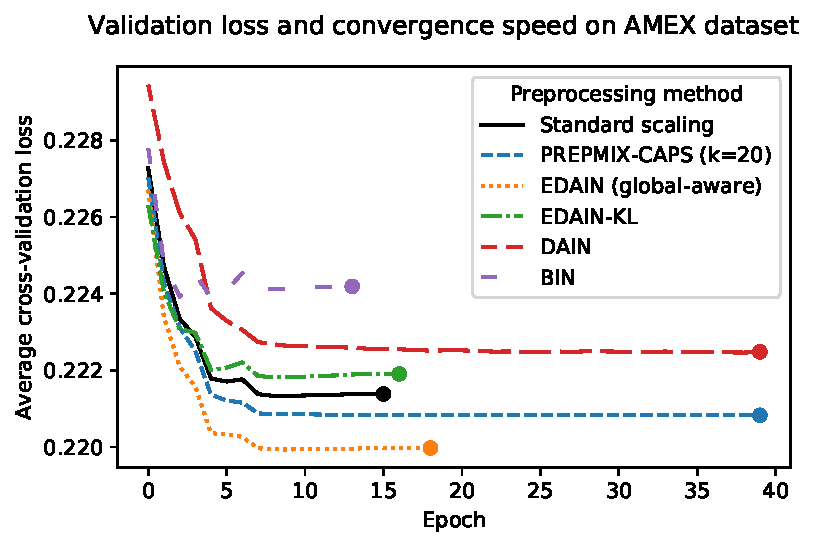
\includegraphics[width=\textwidth]{figures/amex_performance_convergence.pdf}
    \caption{loss}
    \label{fig:amex_performance_loss}
\end{subfigure}
\hfill
\begin{subfigure}[b]{0.99\textwidth}
    \centering
    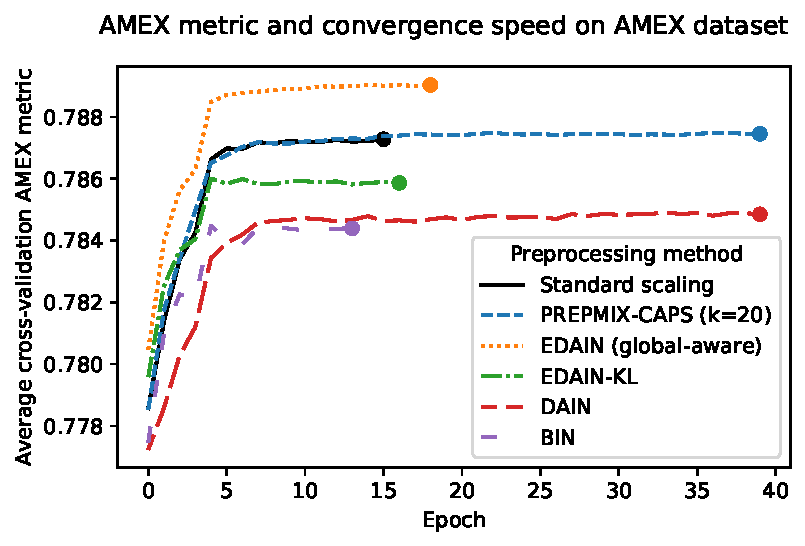
\includegraphics[width=\textwidth]{figures/amex_performance_convergence_metric.pdf}
    \caption{AMEX metric}
    \label{fig:amex_performance_metric}
\end{subfigure}
\caption{Performance and convergence speed. TODO: description, 5 cross-validations, average
value taken. For validations where converged faster, last value used in averaging}
\label{fig:}
\end{figure}

\begin{table}
    \centering
    \begin{tabular}{lll}
        \toprule
        Method & Validation loss & AMEX metric \\
        \midrule
        Standard scaling & $0.2213 \pm 0.0039$ & $0.7872 \pm 0.0068$ \\
        PREPMIX-CAPS (k=20) & $0.2208 \pm 0.0033$ & $0.7875 \pm 0.0053$ \\
        EDAIN (global-aware) & $\mathbf{0.2199} \bm\pm \mathbf{0.0034}$ & $\mathbf{0.7890} \bm\pm \mathbf{0.0078}$ \\
        EDAIN-KL & $0.2218 \pm 0.0040$ & $0.7858 \pm 0.0060$ \\
        DAIN & $0.2224 \pm 0.0035$ & $0.7847 \pm 0.0054$ \\
        BIN & $0.2237 \pm 0.0038$ & $0.7829 \pm 0.0064$ \\
        \bottomrule
    \end{tabular}%
    \label{tab:amex}%
    \caption{Table of asymptotic normal 95\% confidence interval of validation loss and
    AMEX competition metric for the methods considered, confidence interval based on 5 cross-validation folds.}
\end{table}

\begin{table}
    \centering
    \begin{tabular}{lll}
        \toprule
        Method & Cohen's Kappa, $\kappa$ & Average $F_1$-score \\
        \midrule
        Standard scaling & $0.2772 \pm 0.0550$ & $0.5047 \pm 0.0403$ \\
        Min-max scaling & $0.2618 \pm 0.0783$ & $0.4914 \pm 0.0603$ \\
        BIN & $0.3670 \pm 0.0640$ & $0.5889 \pm 0.0479$ \\
        DAIN & $0.3588 \pm 0.0506$ & $0.5776 \pm 0.0341$ \\
        EDAIN (local-aware) & $\bm{0.3836 \pm 0.0554}$ & $\bm{0.5946 \pm 0.0431}$ \\
        EDAIN (global-aware) & $0.2820 \pm 0.0706$ & $0.5111 \pm 0.0648$ \\
        EDAIN-KL & $0.2870 \pm 0.0642$ & $0.5104 \pm 0.0519$ \\
        \bottomrule
    \end{tabular}%
    \label{tab:lob}%
    \caption{Table of asymptotic normal 95\% confidence interval for LOB FI-2010 dataset.}
\end{table}


%%%%%%%%%%%%%%%%%%%%%%%%%%%%%%%%%%%%%%%%%%%%%%%%%%%%%%%%%%%%%
\section{Evaluation methodology}%%%  Evaluation methodology %%
\label{sec:Evaluation methodology}%%%%%%%%%%%%%%%%%%%%%%%%%%%%%

Small introduction

% Sequence model architecture
\subsection{Sequence model architecture}% {{{
\label{sub:Sequence model architecture}

% }}}

% Fitting the models
\subsection{Fitting the models}% {{{
\label{sub:Fitting the models}

Mention scheduling, early stopping, optimizer used, learning rate etc.
% }}}

% Tuning adaptive preprocessing model hyperparameters
\subsection{Tuning adaptive preprocessing model hyperparameters}% {{{
\label{sub:Tuning adaptive preprocessing model hyperparameters}

Details on the tuning for all the methods presented
% }}}

% Evaluation metric
\subsection{Evaluation metrics}% {{{
\label{sub:Evaluation metrics}

% }}}

% Cross-validaiton
\subsection{Cross-validation}% {{{
\label{sub:Cross-validation}


% }}}

%%%%%%%%%%%%%%%%%%%%%%%%%%%%%%%%%%%%%%%%%%%%%%%%%%%
\section{Simulation study}%%%  Simulation study   %%
\label{sec:Simulation study}%%%%%%%%%%%%%%%%%%%%%%%%%

Small introduction, including motivation

% Multivariate time-series data generation algorithm
\subsection{Multivariate time-series data generation algorithm}% {{{
\label{sub:Multivariate time-series data generation algorithm}



% }}}

% Negative effects of irregularly-distributed data
\subsection{Negative effects of irregularly-distributed data}% {{{
\label{sub:Negative effects of irregularly-distributed data}


% }}}

% Preprocessing method experiments
\subsection{Preprocessing method experiments}% {{{
\label{sub:Preprocessing method experiments}



% }}}

%%%%%%%%%%%%%%%%%%%%%%%%%%%%%%%%%%%%%%%%%%%%%%%%%%%%%%%%%%%%%%%%%%%%%%%%
\section{American Express default prediction dataset}%%%  Amex dataset %%%
\label{sec:American Express default prediction dataset}%%%%%%%%%%%%%%%%%%%%

% Description
\subsection{Description}% {{{
\label{sub:Description}

% }}}

% Preprocessing method experiments
\subsection{Preprocessing method experiments}% {{{
\label{sub:Preprocessing method experiments}



% }}}

%%%%%%%%%%%%%%%%%%%%%%%%%%%%%%%%%%%%%%%%%%%%%%%%%%%
\chapter{Discussion} %%%%    Discussion        %%%%
%%%%%%%%%%%%%%%%%%%%%%%%%%%%%%%%%%%%%%%%%%%%%%%%%%%

TODO: introduction to this chapter

% EDAIN
\section{EDAIN}% {{{
\label{sec:EDAIN-discuss}

% }}}

% EDAIN-KL
\section{EDAIN-KL}% {{{
\label{sec:EDAIN-KL-discuss}


% }}}

% PREPMIX-CAPS
\section{PREPMIX-CAPS}% {{{
\label{sec:PREPMIX-CAPS}


% }}}

%%%%%%%%%%%%%%%%%%%%%%%%%%%%%%%%%%%%%%%%%%%%%%%%%%
\chapter{Conclusion} %%%%     Conclusion      %%%%
%%%%%%%%%%%%%%%%%%%%%%%%%%%%%%%%%%%%%%%%%%%%%%%%%%

% Summary
\section{Summary}% {{{
\label{sec:Summary}



Conclusion goes here.



% }}}

% Main contributions
\section{Main contributions}% {{{
\label{sec:Main contributions}

% }}}


% Future work
\section{Future work}% {{{
\label{sec:Future work}

% }}}

% Appendix
% Appendix {{{
\clearpage
 %% reset page counter and start appendix pages with A
\pagenumbering{arabic}
\renewcommand*{\thepage}{A\arabic{page}}

%% Appendix goes here
%\appendix
%
%\chapter{Appendix title}
%
%Appendix goes here.

% }}}

% References {{{
%%References part of appendices
% References: modify the file refs.bib
\bibliographystyle{plainnat}
\bibliography{refs}


% }}}
\end{document}
% vim: set foldmethod=marker:
